\documentclass[11pt, a4paper]{report}
\usepackage{../../styling}

\numberwithin{equation}{section}

\addbibresource{references.bib}

\title{Accumulator System Design for Formula Student Acceleration Event}
\author{Paul Vogelberg}
\date{\today}

\begin{document}

\pagenumbering{gobble}

\maketitle

\tableofcontents
\newpage

\pagenumbering{arabic}
\setcounter{page}{1}

\chapter{Accumulator Design}

\section{Introduction}
In this report, I will present my findings for the design of an accumulator system for the Formula Student electric vehicle, for the theoretical scenario in which the acceleration event is the complete weighting of the competition. The report is structured into two main parts: a technical report detailing the design process and decisions, and a business and entrepreneurial analysis evaluating the commercial viability of the accumulator design.

%TODO: rewrite when fitted within the rest of the group report

\subsection{Project Scope}
The design encompasses the following scope:
\begin{itemize}
    \item Technology down-selection and cell selection for an acceleration-only duty cycle.
    \item Electrical architecture at pack and segment level (busbars, sensing, AMS communication).
    \item Mechanical packaging of segment modules and accumulator container layout.
    \item Analytical verification against power, energy, and voltage-sag requirements.
\end{itemize}

The following items are treated as out of scope for detailed derivation in this document and are stated as future or external work: full BMS firmware implementation, full manufacturing process planning, exhaustive scrutineering documentation, and complete physical test campaign data.

\section{Technology Selection}

\subsection{Design Requirements and Selection Criteria}
Due to the nature of the acceleration-only event, the primary design driver is peak power delivery rather than total energy capacity. This shifts the focus towards technologies with high power density.

To best compare different energy storage technologies, the following selection criteria were established:
(1) power output, (2) total energy capacity, (3) mass, (4) volume, and (5) price.

1. FS Rules regulate the maximum power output of the accumulator system at 80 kW (FS-EV 7.2.4). Power output is assumed constant across the acceleration event due to the negligible time during which traction becomes a limiting factor relative to total event duration.

2. The event duration is estimated as 4 s based on top performances in Formula Student competitions. This conservative estimate ensures adequate margin over typical 3.5 s competitive runs.

Using the fundamental relationship $E = P \cdot t$, the required energy capacity is calculated:
\[E = 80~\text{kW} \times 4~\text{s} = 320~\text{kJ} = 89~\text{Wh}\]

The remaining optimization criteria—mass (3×), volume (1×), and cost (2×)—are minimized to improve vehicle dynamics and overall competitiveness.

\subsection{Energy Storage Media Survey}

The next step is to identify the most suitable energy storage technology. Technologies are shortlisted by lowest mass (the most important factor) for the required power and energy. Table~\ref{tab:storage_comparison} lists the energy and power density for commercially available technologies, with minimum mass estimated for the acceleration-event requirements.

\begin{table}[h]
    \centering
    \caption{Comparative performance of electrochemical energy storage technologies. Values represent commercially available cell ranges \cite{linden2011, miao2019, omar2014, unmannedsystems2024}. Minimum mass calculated for 80 kW power and 89 Wh energy requirements.}
    \label{tab:storage_comparison}
    \footnotesize
    \begin{tabular}{|l|c|c|c|c|}
        \hline
        \textbf{Technology} & \makecell{\textbf{Power} \\ \textbf{Density} \\ \textbf{(W/kg)}} & \makecell{\textbf{Energy} \\ \textbf{Density} \\ \textbf{(Wh/kg)}} & \makecell{\textbf{Limiting} \\ \textbf{Density}} & \makecell{\textbf{Min.} \\ \textbf{Mass} \\ \textbf{(kg)}} \\
        \hline
        Supercapacitor (EDLC) & 1,000 -- 15,000 & 5 -- 10 & Energy & 8.9 \\
        Li-ion Capacitor (LIC) & 2,000 -- 10,000 & 10 -- 20 & Power & 8.0 \\
        High-Power Li-Po & 2,000 -- 8,000 & 100 -- 180 & Power & 10.0 \\
        Lithium Titanate (LTO) & 3,000 -- 5,100 & 50 -- 80 & Power & 15.7 \\
        Lithium Iron Phosphate (LFP) & 200 -- 2,000 & 90 -- 160 & Power & 40.0 \\
        Li-ion (NMC/NCA) & 250 -- 1,500 & 150 -- 260 & Power & 53.3 \\
        \hline
    \end{tabular}
\end{table}

From Table~\ref{tab:storage_comparison}, three main technologies emerge as candidates: supercapacitors (EDLC), lithium-ion capacitors (LIC), and high-power lithium-polymer batteries. These technologies demonstrate the lowest mass requirement for the specified power and energy criteria.

\subsection{Supercapacitor Detailed Analysis}

Supercapacitors are examined as the primary candidate, with lithium-polymer batteries considered later as a performance benchmark.

Supercapacitors store energy as charge electrostatically, allowing for very high power density and rapid charge/discharge cycles. The highest energy density supercapacitors are EDLCs (Electric Double Layer Capacitors).

\begin{equation}
E=\frac{1}{2}CV^2 = \frac{1}{2} C (V_{max}^2-V_{min}^2)
\label{eq:capacitor_energy}
\end{equation}

Where E is energy in joules, C is capacitance in farads, and V is voltage in volts.

From Equation \eqref{eq:capacitor_energy}, voltage sag significantly affects usable energy capacity, necessitating careful consideration of voltage ranges. The upper limit is set by FS-EV maximum voltage regulation (600 V), while the lower limit is determined by inverter and motor minimum operating requirements. Based on the selected powertrain configuration, a conservative minimum voltage of 400 V is assumed.

\begin{equation}
C=\frac{2 E}{V_{max}^2-V_{min}^2}=\frac{2 \cdot 320\text{ kJ}}{600\text{ V}^2-400\text{ V}^2}=3.2\text{ F}
\label{eq:required_capacitance}
\end{equation}

To achieve the required capacitance of 3.2 F at 600 V, we must connect multiple cells together. For equally rated cells, the total capacitance for series connections is given by:

\begin{equation}
C_{series}=\frac{C_{i}}{n}
\label{eq:series_capacitance}
\end{equation}

Where \(C_i\) is the individual cell capacitance, and n is the number of cells in series or parallel.

For the design specification, assuming a cell voltage of 3 V, 200 cells are required in series to reach 600 V. To achieve the required capacitance of 3.2 F, cells must provide 640 F nominal capacitance.

Another key parameter is the Equivalent Series Resistance (ESR), which becomes an important consideration for series-connected supercapacitor cells. The total voltage sag under load is calculated as:

\begin{equation}
V_{sag}=I_{peak} \cdot ESR_{total}=\frac{P}{V_{min}} \cdot ESR_{cell} \cdot n
\label{eq:voltage_sag}
\end{equation}

Where \(I_{peak}\) is the peak current drawn from the pack, and \(ESR_{total}\) is the total ESR of the pack equal to the cell ESR multiplied by the number of cells, n.

\subsection{Supercapacitor Cell Selection}
\begin{table}[h]
    \centering
    \caption{Commercial supercapacitor cell comparison for FS application. Specifications from manufacturer datasheets. Cell count, total capacitance, and voltage sag calculated for 600 V pack with 80 kW peak power at 400 V minimum.}
    \label{tab:supercap_cells}
    \footnotesize
    \begin{tabular}{|c|l|c|c|c|c|c|c|c|c|}
        \hline
        \textbf{ID} & \textbf{Part Number} & \textbf{Cap.} & \textbf{Volt.} & \textbf{ESR} & \makecell{\textbf{Cell} \\ \textbf{Mass}} & \textbf{Cells} & \makecell{\textbf{Total} \\ \textbf{Mass}} & \makecell{\textbf{Total Cap.} \\ \textbf{(Eq.~\ref{eq:series_capacitance})}} & \makecell{\textbf{Volt. Sag} \\ \textbf{(Eq.~\ref{eq:voltage_sag})}} \\
        & & \textbf{(F)} & \textbf{(V)} & \textbf{(m$\Omega$)} & \textbf{(kg)} & \textbf{(n)} & \textbf{(kg)} & \textbf{(F)} & \textbf{(V)} \\
        \hline
        SC1 & \href{https://www.sechsa.com/wp-content/uploads/220106-Sech-datasheet-46mm-cells-1.pdf}{C46W-3R0-0600} & 600 & 3.0 & 0.70 & 0.139 & 200 & 27.8 & 3.0 & 28.0 \\
        SC2 & \href{https://www.gmccsieyuan.com/uploads/C35S-3R0-0600-English.pdf}{C35S-3R0-0600} & 600 & 3.0 & 1.40 & 0.104 & 200 & 20.8 & 3.0 & 56.0 \\
        SC3 & \href{https://en.cda-cap.com/wp-content/uploads/2023/08/bus_elx_ds_4015_CHQ_series.pdf}{CHQ-3R0607R-TW} & 600 & 3.0 & 1.30 & 0.135 & 200 & 27.0 & 3.0 & 52.0 \\
        SC4 & \href{https://datasheets.kyocera-avx.com/AVX-SCC-LE.pdf}{SCCY1KB707SLBLE} & 700 & 2.7 & 1.30 & 0.163 & 223 & 36.3 & 3.14 & 58.0 \\
        SC5 & \href{https://datasheets.kyocera-avx.com/AVX-SCC-LE.pdf}{SCCY83B607SLBLE} & 600 & 2.7 & 1.60 & 0.135 & 223 & 30.1 & 2.69 & 71.4 \\
        \hline
    \end{tabular}
\end{table}

Initial evaluation favored SC3, which offered a good balance between mass and required capacitance while facilitating easy segmentation with its standard 3 V cell voltage. However, further supplier investigation revealed SC2 as a lower-mass alternative. Ultimately, SC1 was selected due to its significantly lower ESR, which minimizes voltage sag during the acceleration event, despite a mass penalty relative to other candidates.

\begin{figure}[h]
    \centering
    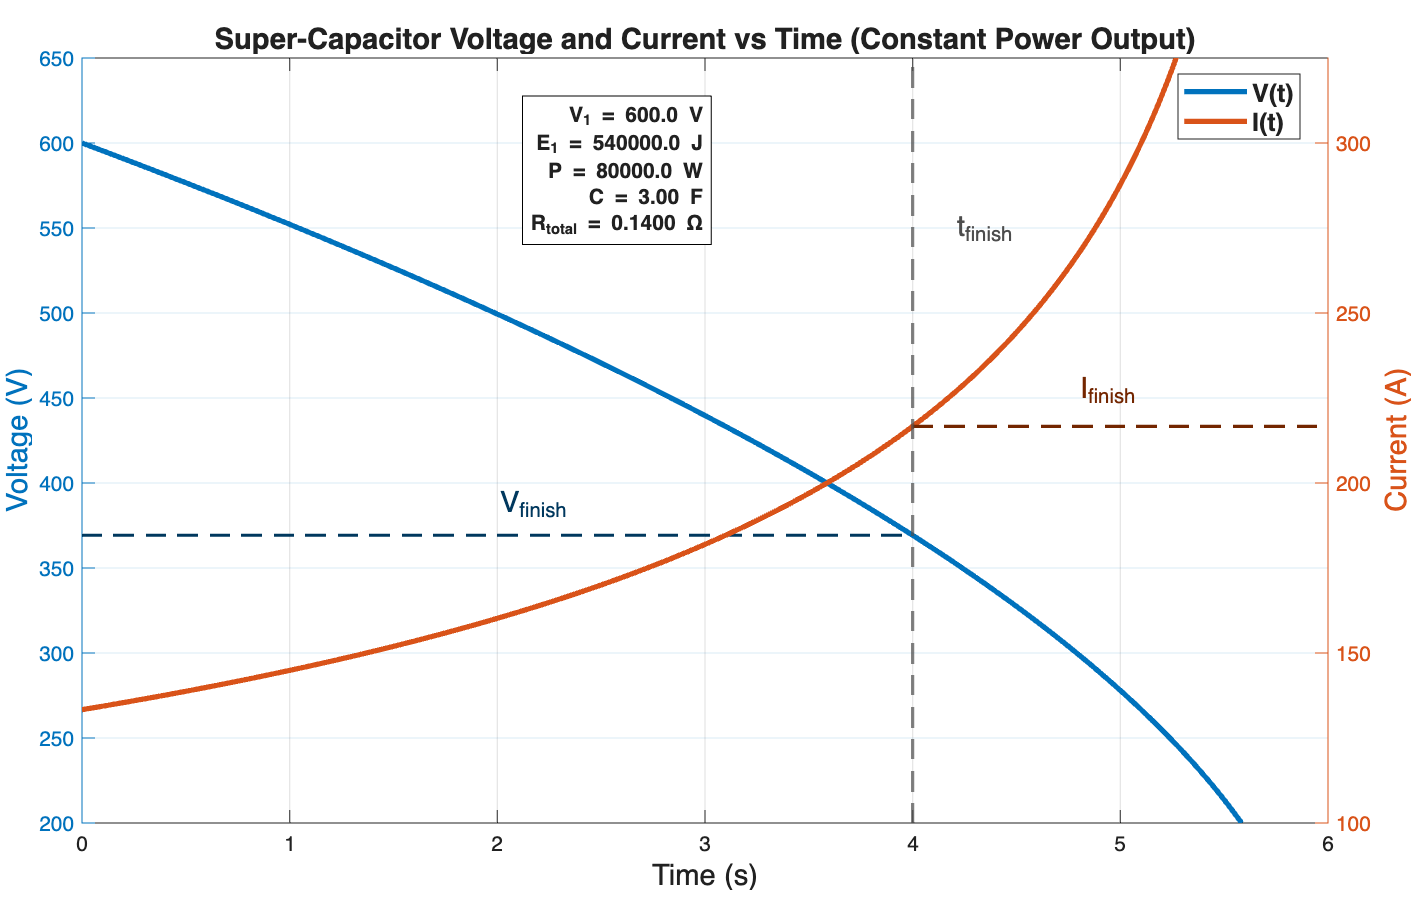
\includegraphics[width=0.8\textwidth]{figures/Supercapcaitor_discharge.png}
    \caption{Selected supercapacitor (SC1) discharge characteristics showing voltage and current evolution over time during constant 80 kW power discharge.}
    \label{fig:supercap_discharge}
\end{figure}
%TODO: Change figure so that Vmin and Imax are numerically labeled and that the Imax line goes to the right axis completely
% TODO: Describe figure \ref{fig:supercap_discharge} and how it validates voltage sag calculation. Also, describe what the straight lines represent
% Maybe make lines thicker and text larger

\subsection{Technology Selection Decision}

The three candidate technologies (EDLC, lithium-polymer, and lithium-ion capacitor) are compared based on mass, volume, cost, performance, and practical availability.

Lithium-ion capacitors (LIC) exhibit significant commercial and data availability constraints. Publicly available cell specifications for 600 V applications are limited. Furthermore, their volumetric capacitance density is inferior to EDLC supercapacitors despite superior energy density. Achieving 600 V would require DC-DC conversion, introducing additional mass and systemic complexity without net benefit. Consequently, LIC technology is excluded from further consideration.

High-power lithium-polymer batteries benefit from widespread adoption in Formula Student and represent mature commercial technology. These cells serve as the performance benchmark for supercapacitor evaluation.

Comparison proceeds via quantifiable metrics of mass, volume, and cost. A weighted scoring system is applied using the following formulation:
\[\text{Score} = \frac{\text{Best Value in Category}}{\text{Component Value}} \cdot \text{Weight}\]

\begin{table}[h]
    \centering
    \caption{Comparison of EDLC supercapacitor and high-power Li-Po battery technologies for acceleration-only application. Weighted scoring system applied with mass (3×), price (2×), and volume (1×) weightings.}
    \label{tab:tech_comparison}
    \footnotesize
    \begin{tabular}{|l|l|c|c|c|}
        \hline
        \textbf{Technology} & \textbf{Cell Component} & \makecell{\textbf{Total Mass} \\ \textbf{(kg)}} & \textbf{Price} & \makecell{\textbf{Volume} \\ \textbf{(L)}} \\
        \hline
        EDLC Cap. & C46W-3R0-0600 & 27.80 & £4,000 & 38.70 \\
        \arrayrulecolor{gray!30}\hline\arrayrulecolor{black}
        LiPo Battery & Melasta SLPB9145180 & 40.00 & £5,500 & 22.00 \\
        \hline
        \hline
        \multicolumn{5}{|c|}{\textbf{Weighted Scoring Analysis}} \\
        \hline
        \textbf{Metric} & \textbf{Weighting} & \textbf{EDLC Score} & \textbf{LiPo Score} & \textbf{Best} \\
        \hline
        Total Mass & 3× & 3.00 & 2.09 & EDLC \\
        \arrayrulecolor{gray!30}\hline\arrayrulecolor{black}
        Price & 2× & 2.00 & 1.45 & EDLC \\
        \arrayrulecolor{gray!30}\hline\arrayrulecolor{black}
        Volume & 1× & 0.57 & 1.00 & LiPo \\
        \hline
        \multicolumn{2}{|l|}{\textbf{Total Score}} & \textbf{5.57} & \textbf{4.54} & \cellcolor{green!20}\textbf{EDLC} \\
        \hline
        \multicolumn{4}{|r|}{\textbf{EDLC Advantage:}} & \textbf{+22.7\%} \\
        \hline
    \end{tabular}
\end{table}

% TODO: Clarify how total mass, volume and price were calculated for Li-Po (source) and supercapacitor. Mass is just cell mass for EDLC

Based on combined quantifiable and performance metrics, EDLC supercapacitors have been selected for this accumulator design. The technology delivers a substantial mass and cost advantage (22.7\% overall scoring benefit) while offering consistent, repeatable performance essential for Formula Student competition requirements.

\section{Electrical System Design}

\subsection{System Architecture Overview}

In \ref{fig:electronics_architecture}, the top-level electrical architecture of the accumulator system is illustrated. The focus of this section will be on the segment electrical design, which includes how the supercapacitor cells are connected via busbars and the sensors which lead to the AMS Slaves. These segments are connected electrically in series together, seperated each by a fuse, and the AMS slaves are daisy-chained together.

The system level accumulator must also have appropriate safety and charging systems, shown on the lower third of the figure, but these are not expanded on in this report as they are not within the scope of the design. The safety system will be designed to meet FS-EV requirements and will include segment fusing, AIR-controlled isolation, and AMS-triggered shutdown on electrical or thermal faults. The charging system will be designed to allow for safe and efficient charging of the supercapacitor pack, with appropriate isolation and control features.

The LV zone includes the BMS Master, connected to the AMS Slaves and itself connected to the Vehicle ECU. 
%TODO: consulte David on chosen ECU model
%TODO: Write something brief about BMS Master.

\begin{figure}[h]
    \centering
    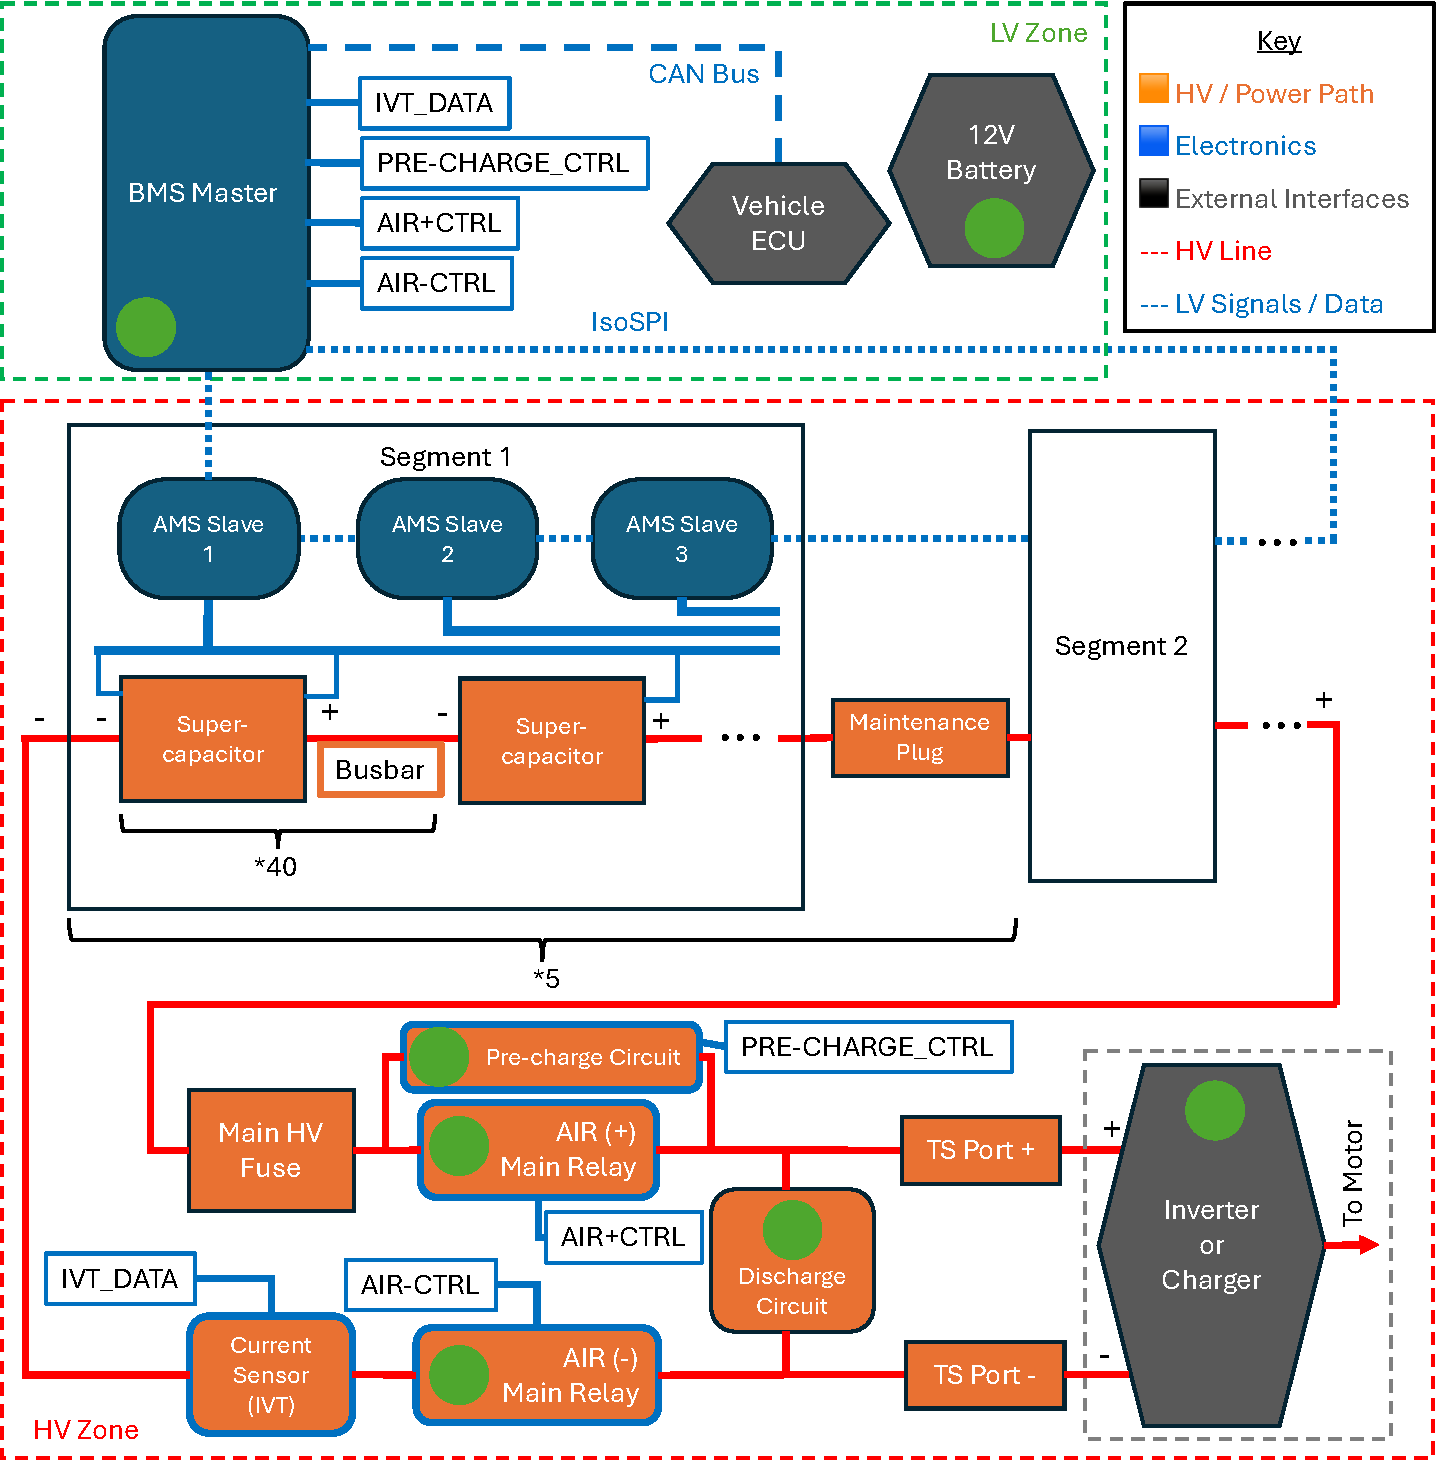
\includegraphics[width=0.9\textwidth]{figures/schematics/Electronics_architecture.pdf}
    \caption{Top-level electrical system architecture showing energy flow from supercapacitor cells through busbars and segments to the inverter, alongside control and communication pathways within the AMS. Green dots represent 12V battery connection}
    \label{fig:electronics_architecture}
\end{figure}

\subsection{Electrical Power Systems}

\subsubsection{Pack Configuration \& Power Distribution}
Supercapacitors are connected via busbars rather than direct cell-to-cell welding for thermal management and assembly accessibility. Busbar material selection minimizes $\rho_{e} \cdot \rho_{m}$, where $\rho_{e}$ is electrical resistivity and $\rho_{m}$ is mass density. Although copper exhibits superior electrical performance, aluminium 1005 was specified for compatibility with aluminium cell terminals and to reduce overall system mass.

Busbar connection area is matched to the terminal cross-section (terminal diameter $d_{t}=10\text{mm}$), with average busbar length $L\approx50\text{mm}$ and target resistance $0.1\text{m}\Omega$ per connection. The required thickness is calculated as:
\[t = \frac{\rho_{e} L}{R d_{t}} = 1.41\text{ mm} \approx 1.45\text{ mm} \text{ (standard 15 gauge)}\]
% Can add a thermal check here as well (even though this is no problem for the busbar design)
%TODO: Insert a simple design of the busbar connection

\subsubsection{Safety \& Protection Systems}
Safety architecture in this design follows standard FS-EV practice: segment fusing, AIR-controlled isolation, and AMS-triggered shutdown on electrical or thermal faults. Detailed circuit implementation is left to the full vehicle electrical integration package.

Grounding is treated as a floating HV system with insulation monitoring against chassis. For EMI robustness, communication uses differential signaling and segregated HV/LV routing.

\subsection{Electronic Monitoring \& Control Systems}

\begin{figure}[h]
    \centering
    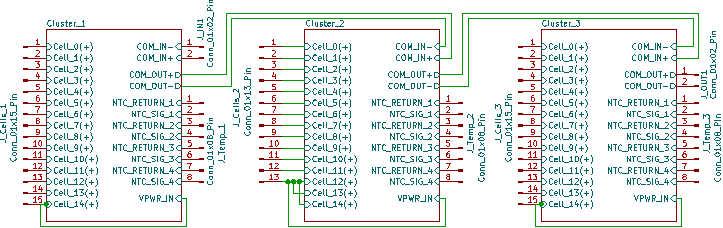
\includegraphics[width=\textwidth]{figures/schematics/PCB.pdf}
    \caption{Complete segment AMS PCB schematic showing MAX17853 configuration, voltage sensing circuits, and cell balancing topology for 40-cell segment monitoring.}
    \label{fig:pcb_schematic}
\end{figure}

The controller IC is powered directly by the local cell stack via the \texttt{VPWR} pins and therefore floats at the segment potential. Functional safety support is provided through open-wire detection using internal current sources at the measurement taps and redundant internal voltage references for ADC cross-checking, aligned with ISO 26262 ASIL-C/D-oriented design practice. The daisy-chain interface follows TPL pin mapping, with \texttt{COM\_IN} receiving data from the lower segment and \texttt{COM\_OUT} forwarding data to the upper segment.

\begin{figure}[h]
    \centering
    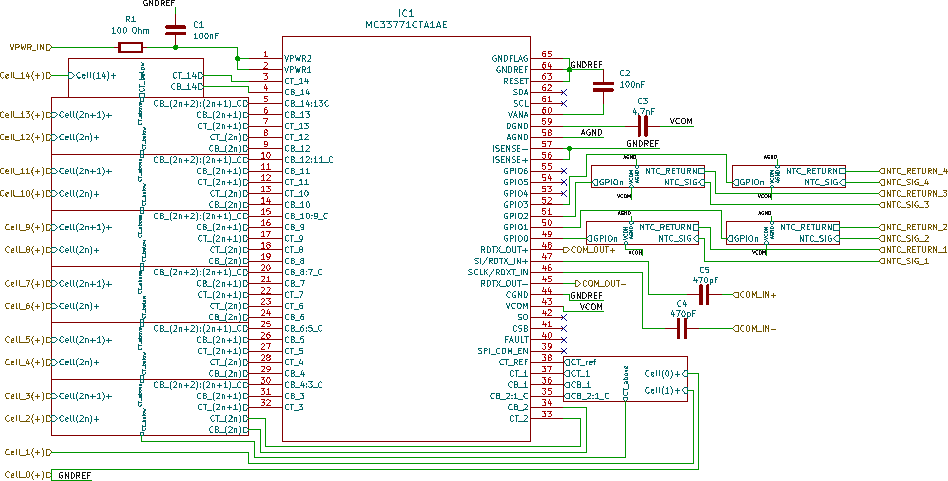
\includegraphics[width=\textwidth]{figures/schematics/PMIC.pdf}
    \caption{Power Management IC (PMIC) circuit providing regulated power supply to the AMS electronics from the high-voltage pack with isolation and protection features.}
    \label{fig:pmic}
\end{figure}

The monitoring network adopts a scalable master-slave topology using NXP MC33771 controllers across all five accumulator segments. Communication is implemented with NXP TPL (Twisted Pair Link) differential signaling, whose current-mode transmission provides strong immunity to inverter-generated EMI. Galvanic domain separation in the daisy chain is maintained using 470 pF high-voltage safety capacitors ($C4$, $C5$), which couple communication across stacked segment voltage domains while blocking DC transfer. On-board routing of \texttt{COM\_IN} and \texttt{COM\_OUT} is implemented as impedance-controlled differential pairs with a 100\,$\Omega$ target to preserve signal integrity.


\subsubsection{Cell Voltage Monitoring}
Cell voltage sensing uses an anti-aliasing filter with $R = 100\,\Omega$ and $C = 47\,\text{nF}$. The corresponding cutoff frequency is
\[
f_c = \frac{1}{2\pi R C} = \frac{1}{2\pi (100)(47 \times 10^{-9})} \approx 33.8\,\text{kHz},
\]
which attenuates high-frequency inverter switching content while preserving measurement bandwidth for pack diagnostics. Passive balancing is implemented through switchable resistors with $R_{bal} = 33\,\Omega$. At a nominal maximum cell voltage of 4.2 V, the balancing current is
\[
I_{bal} = \frac{V_{cell}}{R_{bal}} = \frac{4.2\,\text{V}}{33\,\Omega} \approx 127\,\text{mA},
\]
and the corresponding dissipation per balancing branch is
\[
P_{diss} = I_{bal}^2 R_{bal} = (0.127)^2 \times 33 \approx 0.53\,\text{W}.
\]
This thermal load requires resistor packages with sufficient margin, typically 1210 or 2010 parts rated above 0.75 W for stable operation during balancing intervals.


\begin{figure}[h]
    \centering
    \begin{subfigure}[b]{0.48\textwidth}
        \centering
        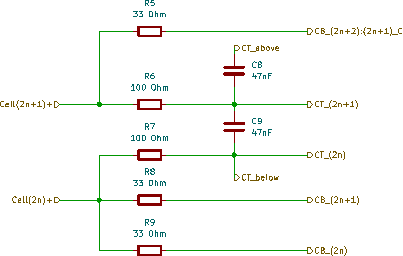
\includegraphics[width=\textwidth]{figures/schematics/VoltageFilter.pdf}
        \caption{Middle filter circuit for noise suppression and signal conditioning in the AMS communication and sensing lines, ensuring accurate voltage and temperature measurements.}
        \label{fig:middle_filter}
    \end{subfigure}
    \hfill
    \begin{subfigure}[b]{0.48\textwidth}
        \centering
        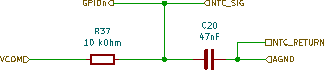
\includegraphics[width=\textwidth]{figures/schematics/TemperatureSensor.pdf}
        \caption{Temperature sensing circuit with NTC thermistor placement strategy and conditioning circuitry for monitoring 30\% of cells per FS-EV requirements.}
        \label{fig:temperature_sensing}
    \end{subfigure}
    \caption{Signal conditioning circuits for AMS monitoring}
    \label{fig:signal_conditioning}
\end{figure}

\subsubsection{Temperature Monitoring}

Temperature channels are conditioned with an RC input filter ($R=10\,\text{k}\Omega$, $C=47\,\text{nF}$) to suppress transient noise that could otherwise cause false over-temperature flags. NTC thermistors are connected directly to MC33771 GPIO measurement channels, and cell temperature is reconstructed from the digitized ratio-metric voltage. The protection strategy applies a hard fault response with AIR de-energization when any monitored cell exceeds the configured threshold of $T > 60^\circ\text{C}$.

%TODO: check through the section and ensure everything is clear, accurate understood (e.g. resistor types)

\subsection{System Integration \& Validation}
% Reivew this section focus.

\subsubsection{Modular Interconnection Design}

\subsubsection{Tolerance Analysis \& Design Margins}

\section{Mechanical Design and Packaging}
The electrical requirement of 200 series-connected cells necessitates segmentation into 5 modules of 40 cells each to maintain voltage domains within FS-EV regulations. All segments are housed within a single Accumulator Container (AC), separated by internal insulating walls and fuse-plug interfaces.

\subsection{Segment Design}

% FIGURE: TODO: Consider an exploded view of CAD rendering of single segment module
\begin{figure}[h]
    \centering
    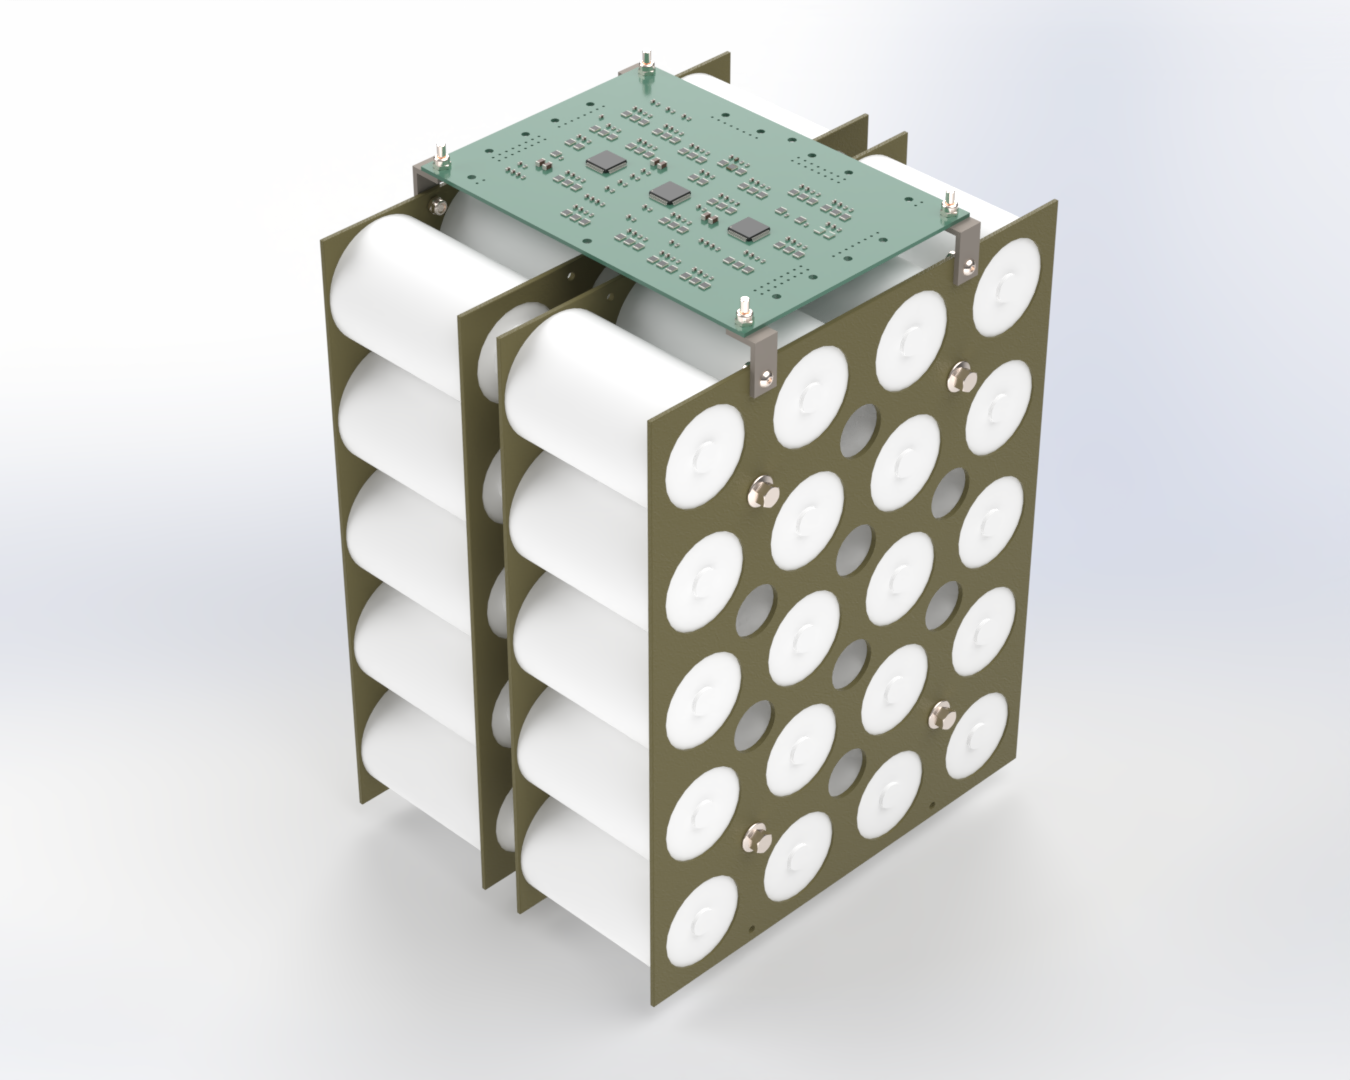
\includegraphics[width=\textwidth]{figures/renders/mainsegment1.png}
    \caption{Accumulator segment design without enclosure and busbar connections.}
    \label{fig:main_segment}
\end{figure}

Segment design prioritizes modularity and replicability, with each segment containing series-connected cells secured by mechanical holders and electrically isolated by spacing. Cells are separated by busbars rather than direct welding to prevent mechanical stress during thermal expansion cycles, ensuring long-term reliability despite increased harness complexity.

Each segment comprises 2 sub-modules of 20 cells each, arranged in a 5×4 rectangular grid. This geometry yields a compact, cuboid form factor. The spacing between sub-modules accommodates placement of thermal and voltage sensing elements and wiring distribution channels.

Packing density optimization typically favors honeycomb arrangements; however, analysis demonstrates that constraining the overall geometry to a cuboid yields only 1\% volume reduction compared to rectangular matrix packing. The rectangular arrangement is consequently selected for its simplicity and superior thermal management properties.

The PCB layout (detailed in Section~\ref{subsec:electrical_design}) is positioned to fit within the segment depth and centered to facilitate harness routing and cell connection while enabling mechanical accessibility via bracket-based mounting to the FR4 matrix board. PCB peripheral spacing accommodates fuse and segment cable routing.

The required fuses for the segment are not showcased, as these will be harnessed to the casing itself, and its positioning cannot be standardised across segments due to the inter-segment casing arrangement. Whilst the busbar design is the same, the mini-PCB busbar design has two main types (see Section 1.3 TODO: add link)), and the arrangement inbetween cells are different to allow for better fuse placement. This will be analysed further in the next section.

% Explain how the segments are designed so that connecting them in different arrangmenets is possible

\subsection{Accumulator Container (AC) \& Integration with Vehicle}

The accumulator positioning within the vehicle is optimized for mass distribution and cabling efficiency. Placement between the driver and motor, below the inverter, achieves complete powertrain separation from the driver compartment, reduces high-voltage cabling mass, and positions the system center of mass near the rear axle per competition requirements. This layout constraint necessitates a 3--2 (top) segmentation configuration as illustrated below.

\begin{figure}[h]
    \centering
    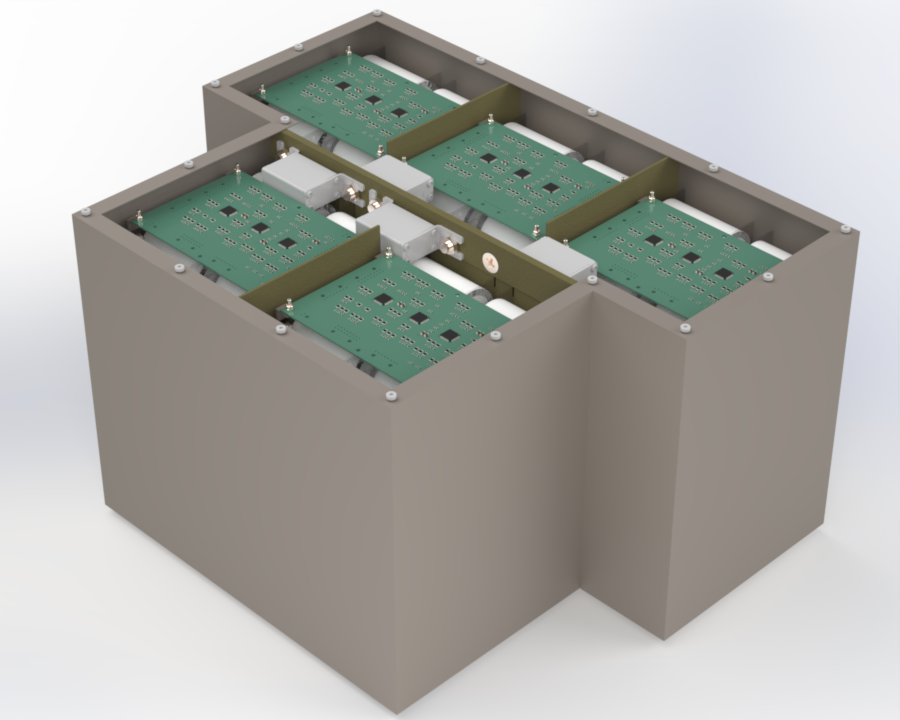
\includegraphics[width=\textwidth]{figures/renders/main4.png}
    \caption{Accumulator design with lid removed for visibility.}
    \label{fig:main_accumulator}
\end{figure}

% TODO: Change Rendering so that the actual floor is at the bottom of the image, then adjust paragraph accordingly

The external casing is fabricated from stainless steel featuring 0.9 mm walls and a 1.2 mm floor panel to meet underbody impact protection requirements. The three-piece assembly—removable bolted lid, welded lower shell, and base floor—enables service access while maintaining structural integrity.

\begin{figure}[h]
    \centering
    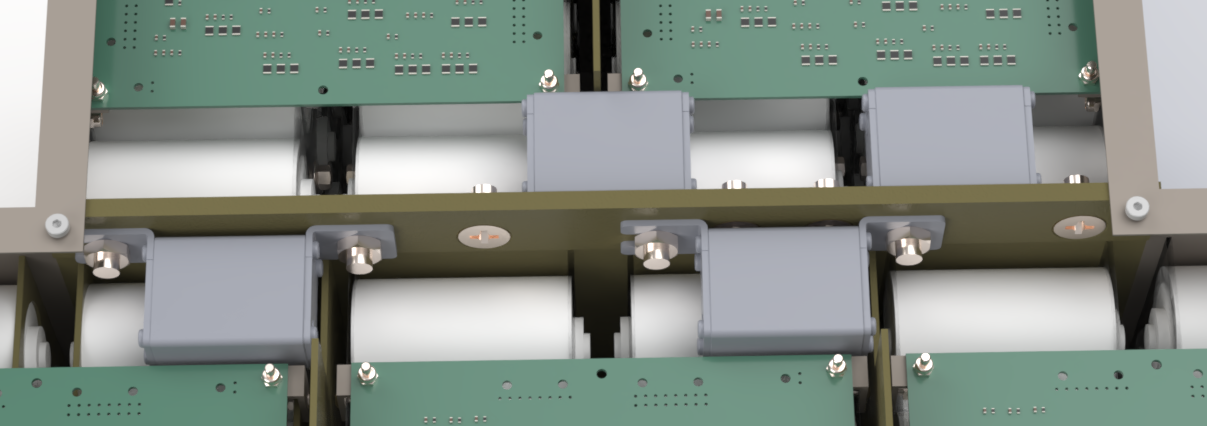
\includegraphics[width=\textwidth]{figures/renders/closeup2.png}
    \caption{Fuse plug placement within the accumulator container.}
    \label{fig:fuse_placement}
\end{figure}

%TODO: Add cabling to the rendering of the close up, to showcase that this has been thoroughly thought through

\begin{figure}[h]
    \centering
    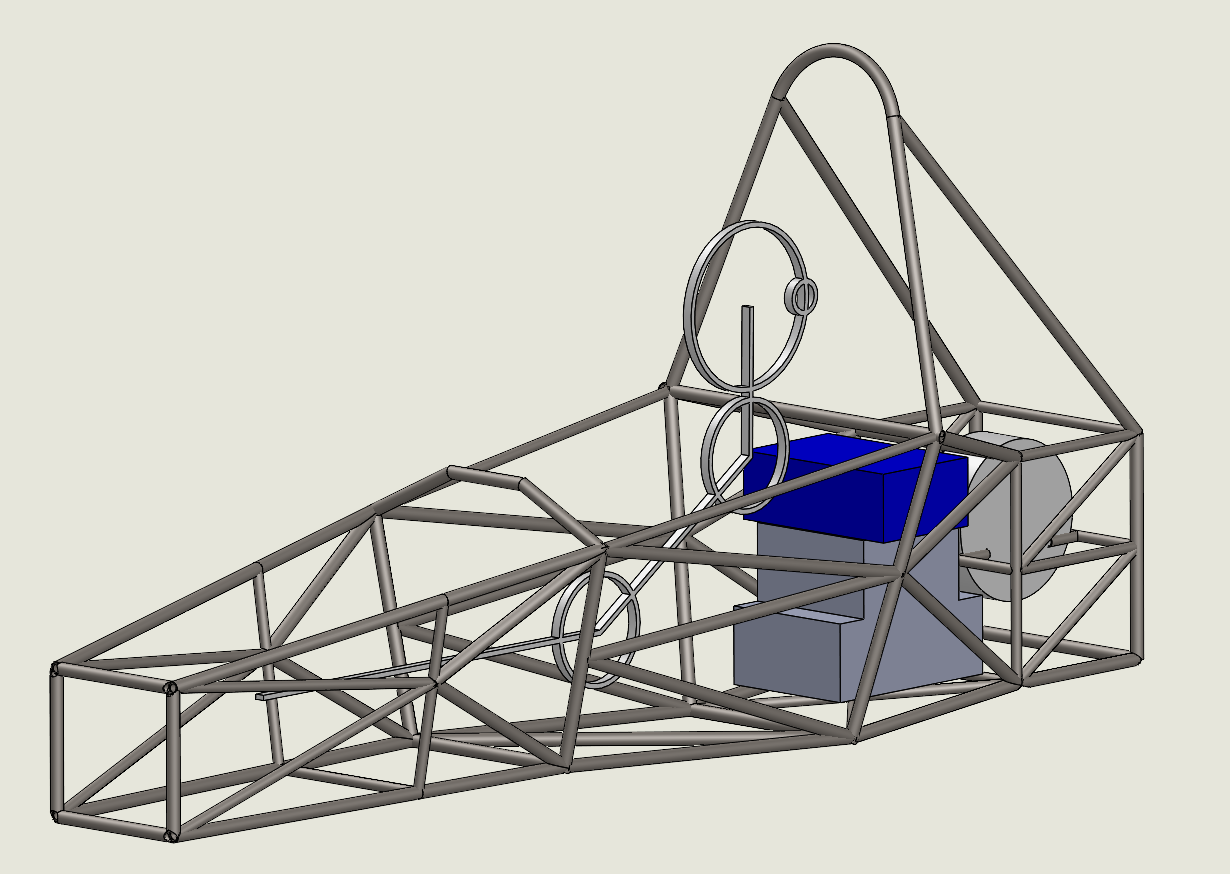
\includegraphics[width=\textwidth]{figures/AccumulatorInCar.png}
    \caption{Accumulator positioned within the vehicle.}
    \label{fig:accumulator_in_car}
\end{figure}

\subsection{Manufacturing Scope}
Detailed manufacturing process planning, quality control workflow, and full BOM costing are not expanded in this report and are deferred to implementation documentation.

\section{Design Verification and Validation}
Verification was performed analytically against the acceleration-event requirements:
\begin{itemize}
    \item Required energy: 
    \item Required capacitance over 600--400 V
    \item Estimated ESR-based sag for selected cells: approximately 
\end{itemize}

The AMS signal conditioning was also checked using first-order circuit calculations % TODO

This level of verification is sufficient for concept selection and architecture justification. Full hardware validation (including insulation, fault-injection, and track testing) is deferred to implementation.

\section{Results and Discussion}

\subsection{Design Criteria Achievement}
The finalized design satisfies all primary performance criteria:
\begin{enumerate}
    \item Peak power delivery: 80 kW sustained across the acceleration event (design specification met).
    \item Usable energy capacity: 320 kJ available over the 600--400 V operating window (design specification met).
    \item Total mass: approximately 38.5 kg (cells only; add 0.5 kg for harness, insulation, fasteners).
    \item Volume: approximately 38.7 L, accommodated within the vehicle's 3--2 segment packaging envelope.
    \item Cost: component cost is favorable relative to lithium-polymer alternatives per Table~\ref{tab:tech_comparison} (EDLC advantage: 22.7\%).
\end{enumerate}

\subsection{Principal Design Trade-Offs}
The fundamental trade-off in supercapacitor selection is voltage sag (determined by ESR) versus total system mass. Minimizing ESR requires larger-diameter cell terminals and busbars, increasing mass; acceptance of higher sag reduces mass but risks insufficient inverter margin. The design balances this by selecting SC1 (lowest ESR, moderate mass) over lighter alternatives (SC2, SC5) that would create unacceptable voltage droop. This selection prioritizes operational robustness and performance consistency over minimal mass.

\subsection{Comparison with Lithium-Polymer Baseline}
Comparison with high-power lithium-polymer technology demonstrates supercapacitor superiority under the specified acceleration-only duty cycle. While Li-Po offers superior volumetric energy density, the supercapacitor architecture provides 22.7\% better overall score when mass, cost, and power delivery are weighted according to Formula Student competition priorities. Additionally, supercapacitor cycle life (>1,000,000 cycles) and run-to-run performance consistency offer competitive advantages unlikely to be replicated by battery chemistry in repeated competitive environments.


\section{Future Improvements and Conclusion}

\subsection{Strategic Refinements for Implementation}
The design establishes a coherent architecture suitable for prototyping and integration. Key refinement priorities for implementation include: (1) detailed thermal analysis during cold-soak conditions to characterize efficiency impact at low ambient temperature; (2) full BMS firmware development including fault detection, cell balancing state machines, and communication protocols; (3) manufacturing partner engagement for cost and lead-time validation; and (4) comprehensive testing including high-voltage insulation verification, fault-injection trials, and track-based dynamic performance characterization.

\subsection{Conclusion}
The accumulator system design successfully combines proven supercapacitor technology with modular electrical and mechanical architecture to meet Formula Student acceleration-event requirements. The analysis demonstrates that EDLC supercapacitors deliver superior performance to lithium-polymer alternatives under the specified duty cycle, with 22.7\% better weighted score across mass, cost, and power density criteria. The design provides clear implementation pathways for component sourcing, manufacturing, and vehicle integration. Subsequent development phases focus on prototype validation, thermal characterization in realistic vehicle operating conditions, and iterative refinement based on test data.


\printbibliography

\end{document}
